

\documentclass[a4paper, 12pt]{report}
%\usepackage[top=1in, bottom=1in, left=1in, right=1in]{geometry} % to change the page dimensions

\usepackage[pdftex]{graphicx}
\usepackage{csquotes}
\usepackage[backend=bibtex,style=numeric,sorting=none]{biblatex}
\usepackage{caption}
\usepackage{subcaption} % for subfigure
\usepackage{hyperref}
\usepackage{amssymb}
\usepackage{tabularx}
\usepackage{multicol}
\usepackage{algpseudocode}
\usepackage{amsthm} % for theorem
\usepackage{algorithm}
\addbibresource{bibliography}

\theoremstyle{plain}
\newtheorem{thm}{Theorem}[chapter] % reset theorem numbering for each chapter

\theoremstyle{definition}
\newtheorem{defn}[thm]{Definition} % definition numbers are dependent on theorem numbers
\newtheorem{exmp}[thm]{Example} % same for example numbers

\usepackage{listings}
\usepackage{color}

\definecolor{dkgreen}{rgb}{0,0.6,0}
\definecolor{gray}{rgb}{0.5,0.5,0.5}
\definecolor{mauve}{rgb}{0.58,0,0.82}

\lstset{frame=tb,
	language=Java,
	aboveskip=3mm,
	belowskip=3mm,
	showstringspaces=false,
	columns=flexible,
	basicstyle={\small\ttfamily},
	numbers=none,
	numberstyle=\tiny\color{gray},
	keywordstyle=\color{blue},
	commentstyle=\color{dkgreen},
	stringstyle=\color{mauve},
	breaklines=true,
	breakatwhitespace=true,
	tabsize=4
}

\begin{document}
\pagenumbering{roman}
\begin{titlepage}
\begin{center}

{\Huge \bfseries
%Inter-Procedural \\
Heap Reference Analysis \\
for Concurrent Programs\\
}~\\[1cm]

% The '~' is needed because \\ only works if a paragraph has started.

{\large \bfseries
B.Tech. Project 2nd Stage Report
}~\\[0.40cm]

{
Submitted in partial fulfillment of the requirements for the degree of
}~\\[0.20cm]

{\large \bfseries
Bachelor of Technology (Honors)
}\\[2.75cm]
\end{center}

\begin{multicols}{2}
\begin{flushleft}
{\large
\textit{Student:} \\
\textbf{Anshul Purohit} \\
\textbf{Roll No: 110050002}
}
\end{flushleft}
\columnbreak
\begin{flushright}
{\large
\textit{Guide:} \\
\textbf{Prof. Uday Khedker}
}
\end{flushright}
\end{multicols}

\vfill

\begin{center}

\includegraphics[width=4cm]{Figures/iitbblack.jpg}~\\[1cm]

{\large
Department of Computer Science and Engineering\\
Indian Institute of Technology Bombay\\
Mumbai 400076, India\\
}

\end{center}
\end{titlepage}
\chapter*{}
\begin{center}
\textbf{Abstract}
\end{center}


This report mainly deals with designing heap reference analysis for concurrent programs in Java. The analysis is both flow-sensitive and context-sensitive at the inter-procedural level. Heap Reference analysis determines a collection of objects pointed to by program variables or their fields. Java implements pointers by references. This report also discusses about analysis techniques for concurrent programs at intra-procedural level and about extending analysis to inter-procedural level using the VASCO tool. In addition to this, this report introduces the notion of handling of thread switching and thread contexts while performing analysis over a data-race free multi-threaded program. This leads to a more precise analysis, as data flow fact propagation along spurious program execution paths are avoided.  

%\addcontentsline{toc}{chapter}{Abstract}
%\begin{center}
{\large \bfseries
Acknowledgement
}~\\[1cm]
\end{center}
\begin{flushleft}
{
I wish to express my sincere gratitude and to my guide, Prof Uday Khedkar for his constant support and guidance throughout the project. I would also like to thank GRC group for all help.
}~\\[1.5cm]
{
Anshul Purohit\\
B.Tech. IV\\
CSE, IIT Bombay
}
\end{flushleft}

\tableofcontents
\pagenumbering{arabic}
\chapter{Introduction}

\section{Background on Program Analysis}

Program Analysis is the set of techniques to get appropriate information about the behavior of programs. Static analysis techniques involve computing approximate information about the program without executing it. In this report, only static analysis techniques would be discussed.  \\ 


Data flow analysis is a technique for gathering information about the possible set of values calculated at various points in a program. The value at each program point is then propagated in the Control Flow graph (CFG) of the program.  The information gathered is often used by compilers when optimizing a program. 

\section{Types of Data Flow Analysis}

A data flow analysis can be either flow-insensitive or flow-sensitive. \\ 

Flow-insensitive analysis:
\begin{itemize}
	\item Ignores the control-flow graph, and assumes that statements can execute in any order.
	\item Rather than producing a solution for each program point, produces a single solution that is valid for the entire program
\end{itemize}
 
Flow-sensitive analysis:
\begin{itemize}
	\item Takes the control
	flow structure of a program into account
	\item Has the computed abstract state that represents different reachable memory states at different program points.
\end{itemize}

A flow-sensitive version of
an analysis is more precise and expensive than the flow-insensitive version. \\

Categorizing according to the direction of traversal of program statements in the CFG, data flow analysis can be broadly of 2 types : forward and backward. Examples of
data-flow analysis are Available Expressions analysis which is a forward data flow analysis
and Live Variables analysis which is a backward data flow analysis. \\

\section{Inter-Procedural Analysis}

Inter-procedural analysis operates across an entire program makes information flow from caller to callee and vice-versa. It extends the scope of data flow analysis across procedure boundaries and it incorporates the effects of procedure calls in the caller procedures, and calling contexts in the callee procedure. A context-sensitive analysis is an \textbf{interprocedural analysis} which reanalyzes callee procedure for each context whereas context insensitive analysis performs analysis independent of calling context.





\section{Concurrency}

For concurrency, we assume the thread model in Java. The high level abstractions of concurrency (such as the DOALL, FORALL, PARBEGIN , PAREND constructs of FORTRAN ) can be modeled in terms of threads and so we use the model of threads to uniformly refer to concurrent programs. The parbegin and parend operations and synchronization during joining of threads will be handled by the Java thread library. The user needs to extend the thread class and define a run method for the object. Invoking the run method on the thread objects starts concurrent execution. For accessing shared data critical sections need to be guarded by the lock and unlock statements. Also we expect a data-race free program as input for analysis.


%\section{Pointers in Java}
%
%Java does not allow the address of a variable to be taken and thus does not allow assignments of the form y = \&x. Java only provided heap-based pointers. Dereferencing is only possible through object fields in Java as the allocated data items do not possess compile-time name in the program. Java does not provide the * operator for dereferencing. 

\section{Problem Statement}  

The idea of the problem statement is to design a framework for carrying out inter-procedural analysis of concurrent programs and then implement heap reference analysis using the framework. The techniques for performing inter-procedural and concurrent analysis is discussed later in the report. Heap reference analysis refers to determining the information like liveness, accessibility and points-to information of reference expressions. Reference expressions, for example \emph{x.lptr.rptr.data} are primarily used to access the objects in the heap. The main focus is on the java model of heap access, in which root variables (variable \emph{x} is on the stack) are stored on the stack. The root variables represent references to memory in heap. Also, root variables cannot be pointed to by any reference.  
 
\section{Organization of the Report}

In this chapter, an introduction to the basics of Data Flow Analysis and its types were described. I have also mentioned about concurrency model and heap accesses for Java. \\

In the subsequent chapters , I will be covering Heap Reference Analysis, Inter-Procedural Analysis and Concurrent Data Flow Analysis respectively. I would then present the tools required for the implementation in the next chapter followed by summary and future work.    
\chapter{Heap Reference Analysis}

Analyzing properties of heap data is not very trivial. This is because the spatial and temporal structure of stack and static data is simple to understand. The stack variables have a compile-time name(alias) associated with it. However, this is not the case with heap data. We need to devise a flow and context sensitive analysis to get information from heap data. 

\section{Difficulties in Analysis of Heap Data}

A program accesses data through expressions having l-values and hence are called access expressions. The l-values can either be a scalar (x), or may involve array access such as \emph{a[2*i]} or can be a reference expression like \emph{x.l.data}. In the case of reference or array, the mapping of the access expression and the l-value may change. The reference expression is primarily used to access the heap.\cite{hra} \\

Heap analysis tries to find out the answer to the questions: 
\begin{itemize}
	\item Can an access expression $a_1$ at program point $p_1$ have the same l-value as access expression $a_2$ at program  point $p_2$.
	\item Can there exist objects in the heap that will not be reachable from the access expressions?
	\item Which of the access links will be live at a particular point?
\end{itemize}
  

\section {Pointer Analysis}

Pointer analysis is a static analysis technique that establishes which pointers or heap references can point to which variables. Pointer analysis collects information about indirect accesses in programs. It can enable precise data analysis and precise inter-procedural control flow analysis. The latter will be used in the VASCO tool that will be discussed later in the report. \\

We have two types of pointer analysis information: points-to analysis and alias analysis. Alias analysis tell if two references point to the same location on the heap. It is transitive in nature. Whereas, points-to analysis tells which memory locations are pointed by references at run-time. \\

Alias information plays an important role in the liveness analysis. Must-alias information is needed to improve precision. May aliases can be found out using information from the points-to analysis. \\

In Java pointers are not created explicitly.\cite{mtpreport} All objects in Java are accessed using references and these references are termed as pointers here. Every time we create an object in Java it creates pointer to the object. This pointer could then be set to a different object or to null, but the original object will still exist. Thus points-to analysis for Java programs identifies the objects pointed to by references at run time. Thus we wish to determine
the objects pointed to by a reference variable or a field. Consider the Java program in Figure 2.1.\\

\begin{figure}
	\begin{minipage}[b]{0.45\linewidth}
		\begin{verbatim}
		
		class A(){}
		class B(){
			public A f;
			public void set(A p)
			{
				this.f = p;
			}
		}
		class C(){
		public B g;
		\end{verbatim}
	\end{minipage}
	\quad
	\begin{minipage}[b]{0.45\linewidth}
		\begin{verbatim}
		
			public void set(B q){
				this.g = q;	
			}
		}
		s1 : A x = new A()
		s2 : B y = new B()
		s3 : C z = new C()
		s4 : y.set(x);
		s5 : z.set(y);
		s5 : A a = z.g.f;
		\end{verbatim}
	\end{minipage}
	\caption{Code to illustrate heap access and points-to analysis}
\end{figure}

In the code given in Figure 2.1, three heap objects pointed to by $x$, $y$ and $z$ are created at $s_1$ , $s_2$ and $s_3$ respectively. We refer to the objects based of their allocation site as $o_1$, $o_2$ and $o_3$. The statement $s_4$ assigns the $f$ field of $o_2$ to point to $o_1$. Similarly, the $g$ field of object $o_3$ is pointed to object $o_2$. Finally the variable $a$ points to the object $o_1$, through reference field indirections.\\      

{\bfseries Liveness and Points-to Analysis} : We can remove some information from the points-to analysis result by considering only information for live pointers. For field references and indirections, liveness is defined using points-to information. \cite{liveness} \\

{\bfseries Points-to graph} in Java contain two types of edges. The first type of edge is to represent the information that reference variable $v$  is pointing to object $o$. The second type of edge represents the field $f$ of $o_1$ pointing to $o_2$. Example of points to graph for the code in Figure 2.1 is shown if Figure 2.2. \\

\begin{figure}
	\centering
	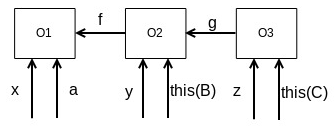
\includegraphics[width=0.6\textwidth]{Figures/rsz_points_to_graph.png}
	\caption{Points to graph for Java program in 2.1}
	\label{fig:points-to java}
\end{figure}

\section{Heap Reference Analysis}

A reference can be represented by access path. In order to perform liveness analysis of heap and identify the set of live links, naming of links is necessary. This is achieved by access path. An Access Path is defined as root variable name following any number of field names and is represented as x $\rightarrow$ n1 $\rightarrow$ n2 ....nk where x is root variable, n1 , n2 .. are field names. If access path \emph{x $\rightarrow$ f $\rightarrow$ d} is live then, the objects pointed to by \emph{x}, \emph{x.f} and \emph{x.f.d} are live. Example of access path is given for the expression \emph{x.left.right.data} in figure 2.3 \\
 
\begin{figure}
	\centering
	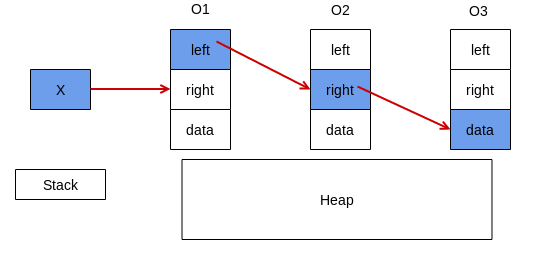
\includegraphics[width=0.6\textwidth]{Figures/hra_access_path.png}
	\caption{Heap reference using access expression \emph{x.left.right.data}.}
	\label{fig:access_path_example}
\end{figure}

An access path can be unbounded in the case of loops. Thus, we require to set a bound on the representation of access paths for liveness information. This is achieved using access graphs which summarizes information based on allocation sites. Access Graph is a directed graph representing access paths starting from root variable. Root node is connected to any number of nodes each having unique labels of form $n_i$ where n is name of the field and i is the program point. Inclusion of program points in access graphs helps in summarization and performing the merge operation.\cite{slides}
Example of access graph and liveness analysis is shown in Figure 2.4. \\

\begin{figure}
	\centering
	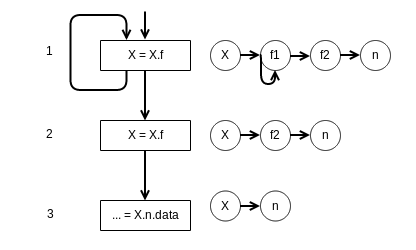
\includegraphics[width=0.6\textwidth]{Figures/heap_summarization_liveness.png}
	\caption{Example of use of access graph and liveness data flow values}
	\label{fig:access_graph_example}
\end{figure}

Availability and Anitcipability analysis of heap data : An access path $\rho$ is said to available at a program point $p$ if the target of each prefix of $\rho$ is guaranteed to be created along each path reaching $p$. An access path $\rho$ is said to be anticipable at $p$ if the target of each prefix of $\rho$ will be dereferenced along every path starting from $p$. Note that access graphs are not needed to carry out to carry out available and anticipable analysis over heap data because the sets are bounded as as result of every control flow path nature of the problems.     
\chapter{Inter-Procedural Analysis}

Inter-procedural Analysis is required to obtain more precise results as it is very common that programs can have multiple function calls. It is essential to consider the effect of function call on the data flow value entering the node. Inter-procedural analysis takes into account call return , parameter passing , local variables of the function, return values and recursion into account. Major issue to be dealt while handling inter-procedural analysis is to deal with calling contexts. Handling concurrency also needs to be supported , which would be discussed in the next chapter. \\


\section{Context Sensitivity}
A context sensitive analysis is an inter-procedural analysis which analyses callee procedure for each context whereas context insensitive analysis performs analysis irrespective of calling context. Context insensitive analysis over-approximates inter procedural control flow which results in imprecision because it takes into account invalid control paths. Each function is analyzed once with single abstract context. Whereas context sensitive analysis is more precise as
it considers the valid inter procedural control flow. \\

Java is an object oriented language supporting features like encapsulation and inheritance. Thus data access is indirect through method calls for each class. So context sensitivity plays a very important role for Object Oriented languages.
     
\section{Call Graph}

Call Graph is graph with nodes and edges in which nodes represent procedures and there is edge from $a$ to $b$ if some call-site at $a$ calls procedure
$b$. Hence this is a static data structure that represents the run-time calling relationships among procedures in program. Soot provides a Spark engine which generates the call graph. VASCO on the other hand returns a much precise call graph, which is generated using liveness based inter-procedural pointer analysis. A thing to note here is that construction of call graph requires inter-procedural analysis and inter-procedural analysis on the other hand requires call graph. An approach to breaking this dependency is to initially approximate the call-graph and in every iteration perform inter-procedural analysis and improve the precision of the call graph.\cite{vasco} \\

Call multi-graph is a directed graph which represents calling relationships between procedures in a program where nodes represent procedures and edges procedure call. A cycle in the call multi-graph denotes recursion. Super graph is another representation in which callsites are connected to the callee procedure entry node and and the exit node of the callee is connected to return node in the caller procedure. \\     

\begin{figure}[here]
	\begin{center}
		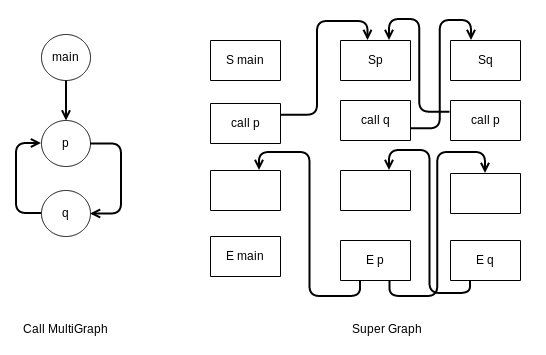
\includegraphics[scale=0.5]{Figures/callgraph.png}
	\end{center}
	\caption{Example of call multi-graph and super-graph}
	\label{fig:call graph}
\end{figure}

Data flow analysis uses static representation of programs to compute summary information along paths. For ensuring safety, all the valid paths must be covered. A valid path is the path which represents legal control flow. Ensuring precision is subject to merging data flow values at shared program points without including invalid paths. For ensuring efficiency, only those valid paths that yield information that affects the summary information should be covered.

\section{Approaches to Inter-procedural Analysis}

In this section approaches to perform inter-procedural analysis is discussed. A very simple approach is to perform procedure in-lining where every procedure call is replaced by the procedure body. This would however only be applicable when target of the call is known and call is not made by pointers or is virtual. However this is not good way to handle recursion as the code size can increase in an unbounded manner. \\

\subsection{Functional approach}

In the functional approach, summary flow functions are computed for each function. The summary flow functions are used as the flow functions for the procedure call. The summary flow function of a given procedure is influenced by the summary flow functions of the callees of $r$ and not by the callers of $r$. Also in the presence of loops or recursion, iterative computation will be needed till fixed point is achieved. Termination is only guaranteed if, lattice is finite.

\subsection{Call Strings Approach}

This is a general flow and context sensitive method. In this approach the call history is stored for information to be propagated back to the correct point. Call string at a program point is the sequence of unfinished calls reaching that point starting from the main procedure call. The data flow equations are changed to incorporate the merging of the data flow values only if the contexts(call strings) are the same. At a call node $c_i$ , $c_i$ is appended to the call-string value at that point. Similarly at a return node the last call site ci is removed. And other data flow values are blocked. For non-recursive programs number of call strings are finite. For recursive programs, number of call strings can be infinite. However, the problem is decidable for finite lattices.

There is an approach of value based termination of call-strings. This method deals with creating equivalence classes. If two call-strings have same data flow values at the start node of the procedure, then they will produce the same data flow values at the return node of the procedure call. Such call strings are grouped into equivalence classes.

An very simple example of call strings method is shown below.\cite{mtpreport}
\begin{verbatim}
public static void main ()
{
	B x;
	// Callsites are appended to the current call string before making call
	C1 : x = deref(f); 
	C2 : x = deref(g);
}
B deref(B a) // c1 [a = f] c2 [a = h]
{
	x.next = a;
	return x;
}
// c1 [ object return would have its next pointed to f] 
// c2 [ object returned would have its next field pointed to h]

\end{verbatim}


\subsection{Value Context Method}

In this method, a combination of tabulation (functional approach) and value based termination (call strings) approach is adopted. The call-stings are partitioned based on the data flow value at the call site. And then analysis of the procedure can then be performed once for each partition. It also combines the two views of contexts: data flow values at call site are stored as value contexts and call strings as calling contexts. Distinct data flow values are maintained for each context of a procedure.\cite{vasco} \\

A value context is defined by a particular data flow value reaching a procedure. It is used to enumerate and store the summary flow function of the procedure in terms of input and output pairs. In order to compute these pairs, data flow analysis is performed within the procedure for each context(input data flow value). The out value of each context is  initialized with the top element. This approach also maintains a context transition table which allows flow of information along inter-procedurally valid paths. Transitions are recorded in the form (($X$,$c$) , $Y$) where $X$
represents calling context, $c$ represents call site and $Y$ represents callee context. Hence when analysis of callee procedure completes where to return is
identified by context transition table. Therefore propagation to valid path is guaranteed. \\

When a new call to a procedure is encountered, the context table pairs are consulted to decide if the procedure needs to be analyzed again. If it was already analysed once for the input value, output can be directly processed else a new context is created and the procedure is analysed for
this new context.

\section{Example of value context method}

\begin{figure}[here]
	\begin{center}
		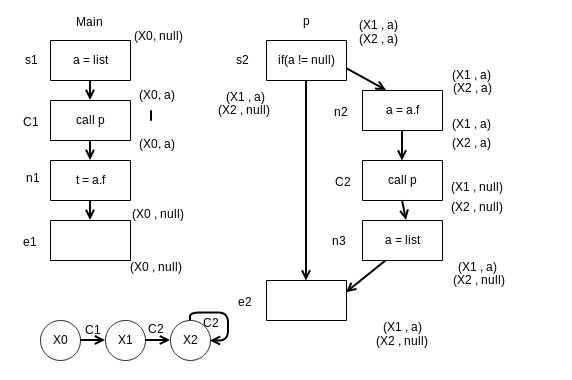
\includegraphics[scale=0.5]{Figures/interproc_example.png}
	\end{center}
	\caption{Example of value-context based IP analysis}
	\label{fig:extreme}
\end{figure}

This is an example of an inter-procedural heap liveness analysis. We wish to find out if a is live before and after the statement $C_1$ The procedure p is recursive and gets called with two different contexts $X_1$ and $X_2$ as shown in the context transition diagram as well. \\ 

The analysis starts with the intial context $X_0$ at statement e1 in main with the value null . The in value of $n_1$ is becomes $a$ as \emph{a.f} is being set to $t$ in the statement. On the next node $C_1$, we have a function call to $p$. So a new value context $X_1$ is created with input $a$ and value $null$ and the transition from X0 to X1 is noted. Now in $X_1$ context, node $n_3$ is processed followed by $c_2$, which creates another value context $X_2$ for procedure $p$ with input $null$ with value $null$. The transition $X_1$ to $X_2$ is also recorded in the context transition table. \\

In the context $X_2$, node $c_2$ is evaluated. Since there is already a context for input value $null$ we take its out value to be $null$ (the top value of the lattice). Thus, the in values of $C_2$ and $n_2$ are set to $null$ and $a$ respectively. Since $s_2$ does not kill the access path $a$, the output value of context $X_2$ is set to $a$. \\

The callers of $X_2$ are $X_1$ and $X_2$ itself. Both these contexts are now added to the work-list for processing. The only change for context $X_2$ is in the call statement $c_2$ whose in value is now set to $a$. On evaluating context $X_1$, we similarly get its output value to be $a$. After this step, the statement $C_1$ in context $X_0$ gets the in value assigned to be $a$, which gets killed in $s_1$.  \\

%X3,c2 is picked up for processing and this time the correct exit value of X2 i.e u+v- is used and so the out value of X3,c2 becomes a-b+c-. However the values do not change for its successor. Thus no more nodes of X3 need to be expanded. The process continues with X1,c2. It's out value comes out to be a+b-c- as the exit value of X2 is u+v-. X1,n3 is then picked up. The sign of c is found out to be negative and this propagates to the end of the procedure. The exit values of X1 becomes a+b-c-. And now X0,c1 is added to the work list for processing and thus q is found out to be negative. \\
%
Value based contexts are used as a cache table for distinct call sites apart from terminating analysis of recursive procedures. 



\chapter{Analysis for Concurrent Programs}

We will be using the technique mentioned in the paper Dataflow Analysis for Datarace-Free Programs\cite{Arnab2006}. This technique when given a sequential data-flow analysis produces an efficient and fairly precise analysis for concurrent programs. The criteria to be met for applying this analysis is that data-flow fact should  be dependent on the contents of the associated lvalues (expression referring to memory location at runtime). Sequential analysis like null-pointer analysis, interval analysis and constant propagation. In terms of precision of the data-flow facts, useful information will be derived at program points where the lvalue is read.\cite{Arnab2006} \\

The main challenge in converting the analysis from sequential to concurrent programs is that propagating data-flow values such that all the possible concurrent executions of the thread are taken care of. In this technique, the synchronization structure of the program is made use of to propagate data-flow values. The main insight used is that the data-flow values are only propagated between threads at the lock and unlock points in threads for access to critical sections. Also this approach will not work for programs containing data race. \\

\section{Memory Model and Data Races}

We will model the notion of concurrency in programs using threads at the moment. The shared variables in the thread will be accessed inside a pair of lock and unlock statements. Note that, this only covers the case in which only one thread can execute in the critical section. We have not modeled the case of general semaphores in which multiple threads can execute inside the critical sections. \\

A memory model specifies the interactions of threads with memory and its shared use. Thus , memory model specify the constraints on data access and conditions on how data written by one thread is accessible to other threads. Happens before is the memory model described in the paper and thesis on Concurrent Program analysis. \\ 


The happens before memory model is based on the happens-before relation which relates the happenings of two events such that if one happens before the other, it should be reflected in the results. That is if statement A occurs before statement B then the memory written by statement A is visible to statement B. \\
There are three components of the happens before memory model.
\begin{enumerate}
	\item Program Order: It is generally used to refer to the order of statement in a thread as they appear in the program. However the formal definition of program order is the intra-thread order during the execution of the program.
	\item Synchronizes-with Relation: This relation is defined over synchronization relations which are lock, unlock (for acquiring/releasing locks), spawn, join (to synchronize creation/endind of multiple threads), start, end(first/last statement of a thread). The synchronizes-with relation is defined from
	\begin{itemize}
		\item Lock statement to all previous unlock statements
		\item A begin statement to the spawn statement of the thread
		\item Join statement to the end statements of all the threads synchronized
	\end{itemize} 
	\item Happens-Before Order: Statement  a happens before statement b if one of the following hold
	\begin{itemize}
		\item a appears before b in the program order
		\item b synchronizes-with a
		\item b can be reached transitively using happens-before relation from a.
	\end{itemize}   
\end{enumerate}
 
\begin{figure}
	\centering
	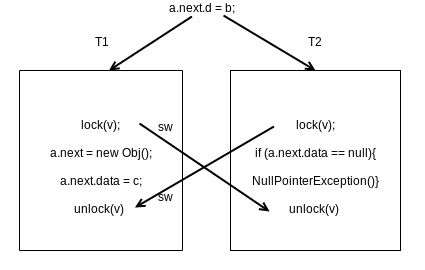
\includegraphics[width=0.6\textwidth]{Figures/sync_threads.png}
	\caption{Happens Before memory model with thread synchronization}
	\label{fig:happensbefore1}
\end{figure}


\begin{figure}[b]
	\centering
	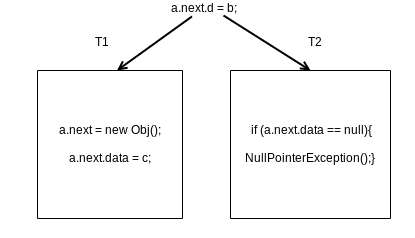
\includegraphics[width=0.5\textwidth]{Figures/sync_no_lock.png}
	\caption{Happens Before memory model without thread synchronization}
	\label{fig:happensbefore2}
\end{figure} 
 
Consider the example presented in Figure 4.1. We have an example of 2 threads executing the critical section. Assume that \emph{a.next} was initially pointing to an object $o_i$ on the heap which contains non-null data. We need to check if the exception in $T_2$ can be thrown. Applying the happens-before relation, we can find out this will never be the case. The synchronization of locks and unlocks always prevents the possibility of \emph{a.next} pointing to a dynamically created object with \emph{null} when the \emph{if} condition in $T_2$ is checked, irrespective of any possible thread scheduling. The exception would only have been raised if the statement 2 of T \\

Now consider the case given in Figure 4.2. It has the same statements but does not contain proper locking and hence no synchronization edges. So in this case all the actions in T1 need not happen before the evaluation of the condition. The exception can now thrown be in case the execution order is {($T_1$,$s1$),($T_2$,$s2$)}. This necessitates data race free program as input to the analysis.\\


Data Race : A data race occurs when two or more threads can access shared data at the same time and try to change it at the same time. Also the order of access among the threads will not be known, so both the threads are racing to access or modify the shared data. Formally, a data race is said when

\begin{enumerate}
	\item Two or more threads access the same memory location concurrently
	\item At least one of the accesses is a write
	\item he threads are not using any exclusive locks to control their accesses to that memory.
\end{enumerate}

Data race can be defined in terms of happens before relation. Two statements are said to be conflicting/racy if neither a happens before b or b happens before a. We will only deal with programs which are data race free. 

\section{Concurrent analysis technique}

Arnab De has explained his approach to concurrent data flow analysis\cite{Arnab2006} by giving example of access path based null-pointer analysis. He argues that the data-flow value is true only before the statement where the corresponding access path/lvalue is relevant. \\

The first step in the analysis is to add edges between nodes of control flow graph representing different threads. These edges map to the synchronize-with edges in the happens before memory model. Hence, the name sync-CFG is given to this control flow graph. The edges are added from the spawn statement to the first statement of each thread, from the unlock statement to lock statement if they access the same lock variable and  belong to different threads. In the next step sequential data flow analysis is performed on the syn-CFG. The synchronization edges have identity flow functions. The example of the access-path based null pointer analysis inspired from\cite{Arnab2006} is in Figure 3.1 \\

\begin{figure}
	\centering
	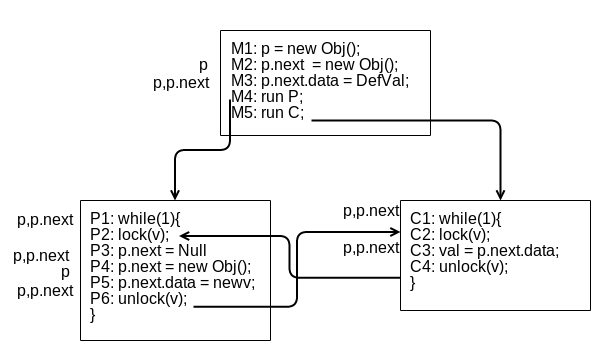
\includegraphics[width=0.6\textwidth]{Figures/concurrent_analysis.png}
	\caption{Heap Access path based null pointer analysis}
	\label{fig:nullpointeranalysis}
\end{figure}


In Figure 3.1 the synchronization edges are added to generate the sync-CFG.It also shows access paths to memory locations which are discovered to be not null by the analysis. The values are marked in italics for each corresponding statement. As p.data is non-null at point $M_5$ in the main thread before spawning the cons thread, this value gets propagated to the first instruction $C_1$ of the cons thread though one of the added edges, and from there to the lock instruction at $C_2$. Similarly, although \emph{p.next} is set back to non-null at $P_4$ before the unlock, despite being set to
null at $P_3$ in the prod thread. This fact also gets propagated to the lock statement of the cons thread through the edge from $P_6$ to $C_2$. As p.next is not null in both the paths joining at $C_2$, we can conclude \emph{p.next} to be non-null before the lock statement in all executions by the merge operation. \\

An important point to note about this technique is that, it may compute incorrect values at program points not containing access paths. For all data-race free programs, relevant statements will occur in the lock-unlock regions. Those statements containing access path or reference expression are considered relevant. In the given example $C_1$ is not a relevant statement and the data flow value \emph{p.next} is incorrect considering the program execution order [$P_3$ $C_1$]. %An example that can be designed to provide as input for concurrent heap liveness analysis is shown in Figure 4.4. 

\section{Concurrent Heap Liveness Analysis}

Consider the Example shown in Figure 4.4, showing the first iteration. Heap  liveness analysis is a backward flow problem. Figure 4.5, 4.6,4.7 shows the data flow values after iterations 2,3 and 4 respectively. At the beginning of $s_1$ in Thread 1, the live access path are \emph{x.f1.r}, \emph{x.f1.f2.r}. This is approximated by the access graph shown in Figure 4.7. Access graph representation is essential to represent finitely, the access paths(especially in the case of presence of loops). The synchronization edges introduce a structure similar to loops in the sync-cfg. Thus paths like \emph{x.f1.f2.f1.r} and \emph{x.f1.f2.f1.f2.r} are marked out to be live. We will obtain extra spurious live access paths by adding sync-edges, however the access graph will contain all the valid live paths at a point inside the lock-unlock statements. Also , note that at the start of the main statement, \emph{x.f1.r},\emph{x.f2.r}. \emph{x.f1.f2.r} and \emph{x.f2.f1.r} paths are live.\\

Figure 4.8 shows the heap liveness analysis performed without adding the synchronization edges in the cfg. This will just mark out the access path \emph{x.f1.r} live at the starting of $s_1$ in Thread 1. The absence of synchronization edges misses out the liveness of the access path \emph{x.f1.f2.r} at the starting of $s_1$ in Thread 1. The access graph at the start of the statement main is same even without the effect of synchronization edges for this example. Even without synchronization edges,the access paths \emph{x.f1.r},\emph{x.f2.r}. \emph{x.f1.f2.r} and \emph{x.f2.f1.r} are live. \\

Figure 4.9 illustrates the an input cfg that needs to be given as input to the concurrent heap liveness analysis. We also  need to handle procedure calls inside the lock-unlock statements, using the value contexts method. \\

In the next chapter we will be discussing the problems with this analysis method. The fact that analysis without adding synchronization edges gives better liveness data flow value, highlights that there are some problems with this analysis. We will discuss them in greater detail in the next chapter. 

\begin{figure}
	\centering
	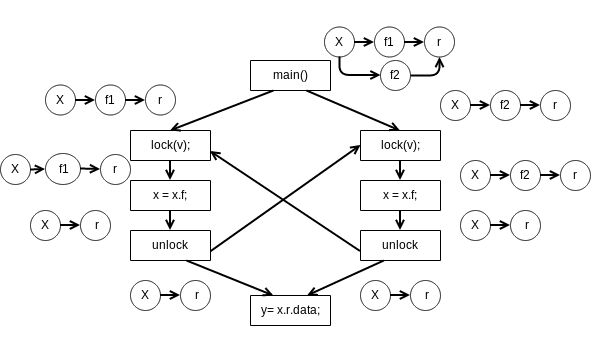
\includegraphics[width=0.8\textwidth]{Figures/conc_analysis_itr1.png}
	\caption{Concurrent Heap liveness analysis iteration 1}
	\label{fig:nullpointeranalysis}
\end{figure}

\begin{figure}
	\centering
	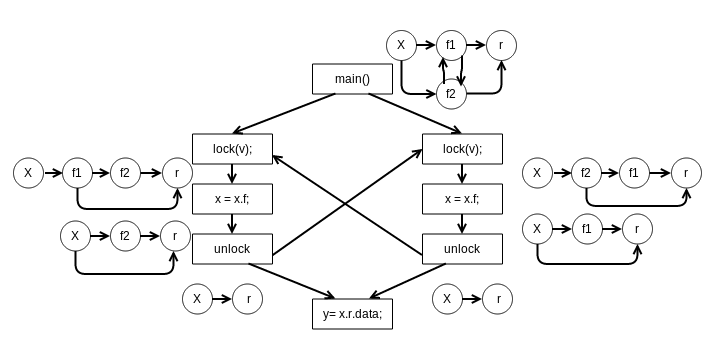
\includegraphics[width=0.8\textwidth]{Figures/conc_analysis_itr2.png}
	\caption{Concurrent Heap liveness analysis iteration 2}
	\label{fig:nullpointeranalysis}
\end{figure}

\begin{figure}
	\centering
	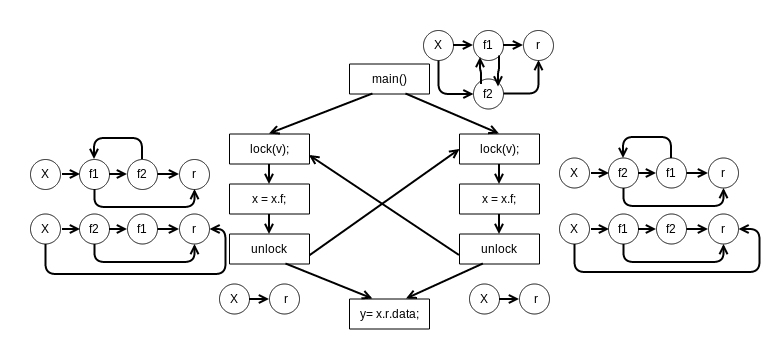
\includegraphics[width=0.8\textwidth]{Figures/conc_analysis_itr3.png}
	\caption{Concurrent Heap liveness analysis iteration 3}
	\label{fig:nullpointeranalysis}
\end{figure}

\begin{figure}
	\centering
	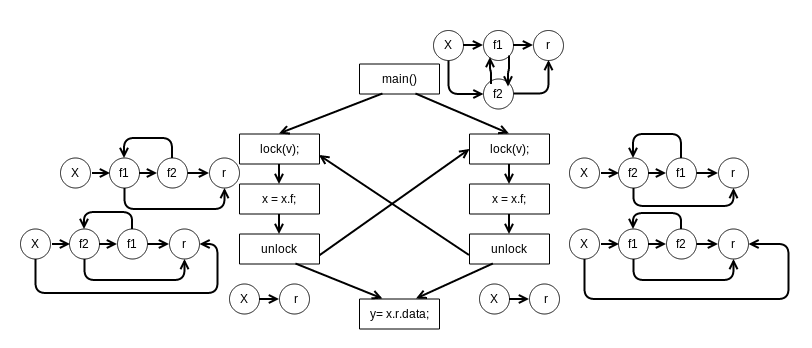
\includegraphics[width=0.8\textwidth]{Figures/conc_analysis_itr4.png}
	\caption{Concurrent Heap liveness analysis iteration 4}
	\label{fig:nullpointeranalysis}
\end{figure}

\begin{figure}
	\centering
	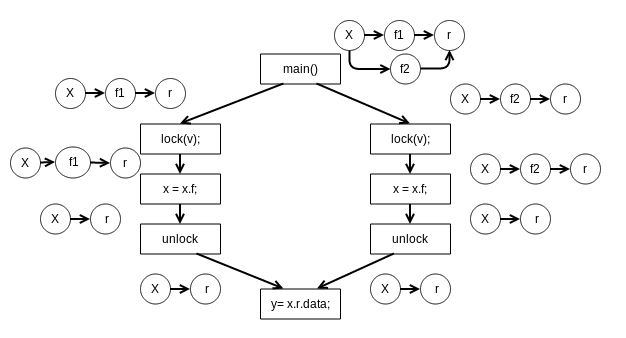
\includegraphics[width=0.8\textwidth]{Figures/conc_analysis_incorrect.png}
	\caption{Concurrent Heap liveness analysis without synchronization edges}
	\label{fig:nullpointeranalysis}
\end{figure}

\begin{figure}
	\centering
	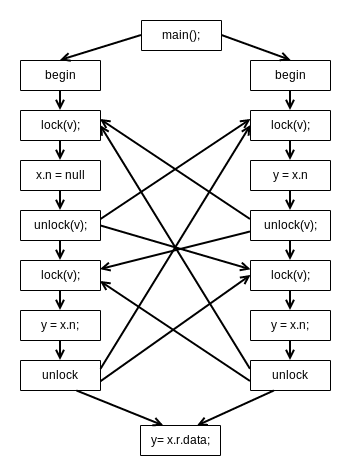
\includegraphics[width=0.5\textwidth]{Figures/hra_live_concurrent.png}
	\caption{Concurrent Heap liveness analysis input}
	\label{fig:nullpointeranalysis}
\end{figure}     


\chapter{Problem with the Concurrent Analysis Method}

The analysis technique presented in the previous chapter, propagates the data flow values across inter-thread edges in the same way as it propagates the data flow flow along inter-thread edges. Consider the output of heap-liveness analysis technique on the same example of the previous chapter. The figure 5.1 is the final data flow value obtained after convergence. \\

\begin{figure}
	\centering
	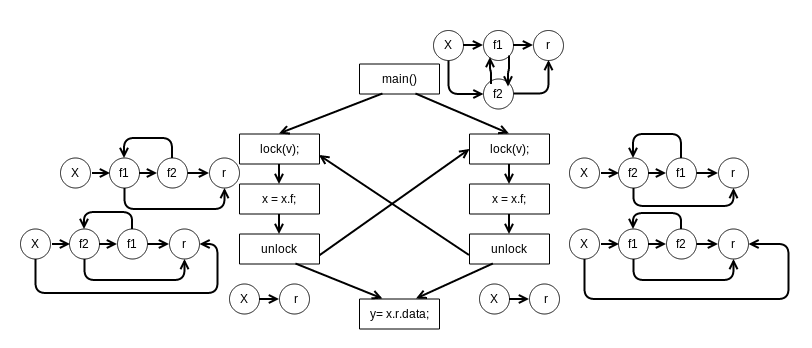
\includegraphics[width=0.8\textwidth]{Figures/conc_analysis_itr4.png}
	\caption{Example of the concurrent analysis technique}
	\label{fig:ch5example}
\end{figure}


At the program point containing the main statement, the possible live links would be \emph{x.f1.f2.r} or \emph{x.f2.f1.r}. However the final data flow value  obtained at the main statement includes access links \emph{x.f1.r}, \emph{x.f2.r} , \emph {x.\{f2.f1\}\textsuperscript{+}.r}, \emph{x.\{f1.f2\}\textsuperscript{+}.r} which are imprecise values. The major source of error is due to the transitions from node $f_1$ to $f_2$ and from $f_2$ to $f_1$ in the access graph. \\

The imprecise data flow values are a result of taking into account execution of critical sections more than once. The thread synchronization edges introduce loops in the program graph. The current method treats these thread synchronization edges as loops and continues propagation of the facts until a converged value is obtained (as seen in the previous chapter). \\

\section{Execution of Critical Sections}

The execution of a multi-threaded program is an interleaving of statements of the multiple threads. Critical sections are regions where the shared variables are accessed under mutual exclusion. Thus there is a need to identify the critical sections that only execute once. The analysis to figure this out is thread independent. Note that a critical section can only be executed once if there are no backward program edges from a statement after unlock(v) to one before lock(v). For such critical sections we need to keep track to thread switches encountered while performing the analysis. In the example figure 5.1, if the critical section of thread 1 is analyzed and the data flow value is transferred to thread 2 for analysis along an inter-thread edge, it is required to ensure that data flow value in not transferred back to thread 1 after analysis of thread 2 critical section. \\


For handling such cases, we need to examine the presence of loops within each thread. 
\begin{itemize}
	\item If there is no loop within and across a critical section, it can only be executed once.
	\item If a loop is present within a critical section, even then the critical section can be executed only once. This is so because if 1 thread enters a critical section, all other threads wait until the this thread completes executing the loop inside the critical section.
	\item It a loop is present across a critical section in a thread, then the critical section can be executed zero or more number of times. Apart from that we may have execution of other critical sections between two executions on this critical section (inter-leaving) possible.
\end{itemize} 

Thus we need to figure out how to store the thread switchings in an access graph. One possible way is to store thread id corresponding to every edge in the access graph. Once each edge is labeled, we need to identify which paths are possible with respect to the execution semantics. For instance, as pointed above, we cannot allow paths with multiple thread switches into a critical section which can only be executed once. We will now need to examine all the paths where the execution semantics are followed. \\

\begin{figure}
	\centering
	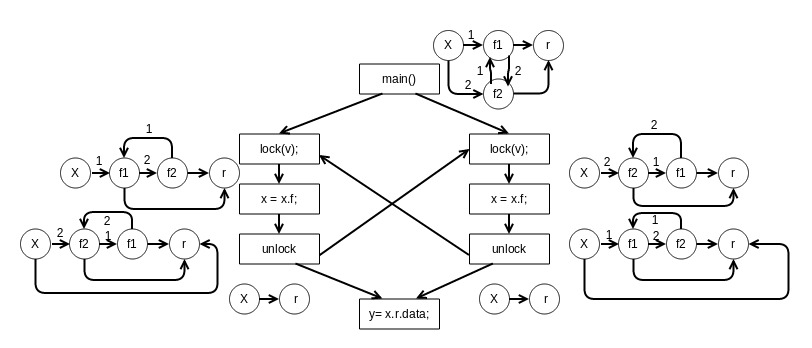
\includegraphics[width=0.8\textwidth]{Figures/conc_analysis_thr_itr3.jpg}
	\caption{Concurrent Heap liveness analysis example. Note that edges are marked by thread id}
	\label{fig:threadidanalysis}
\end{figure}

In figure 5.2, at the point main, we obtain an access graph which includes multiple access links. By imposing the restrictions that concurrent sections in thread 1 and 2 can only be executed once, we can discard all the access paths that contain more than 1 edges labeled 1 or 2. This way we can ensure that we get precise links.

Suppose we take another example in which we have an inner loop in a critical section. 

\begin{figure}
	\centering
	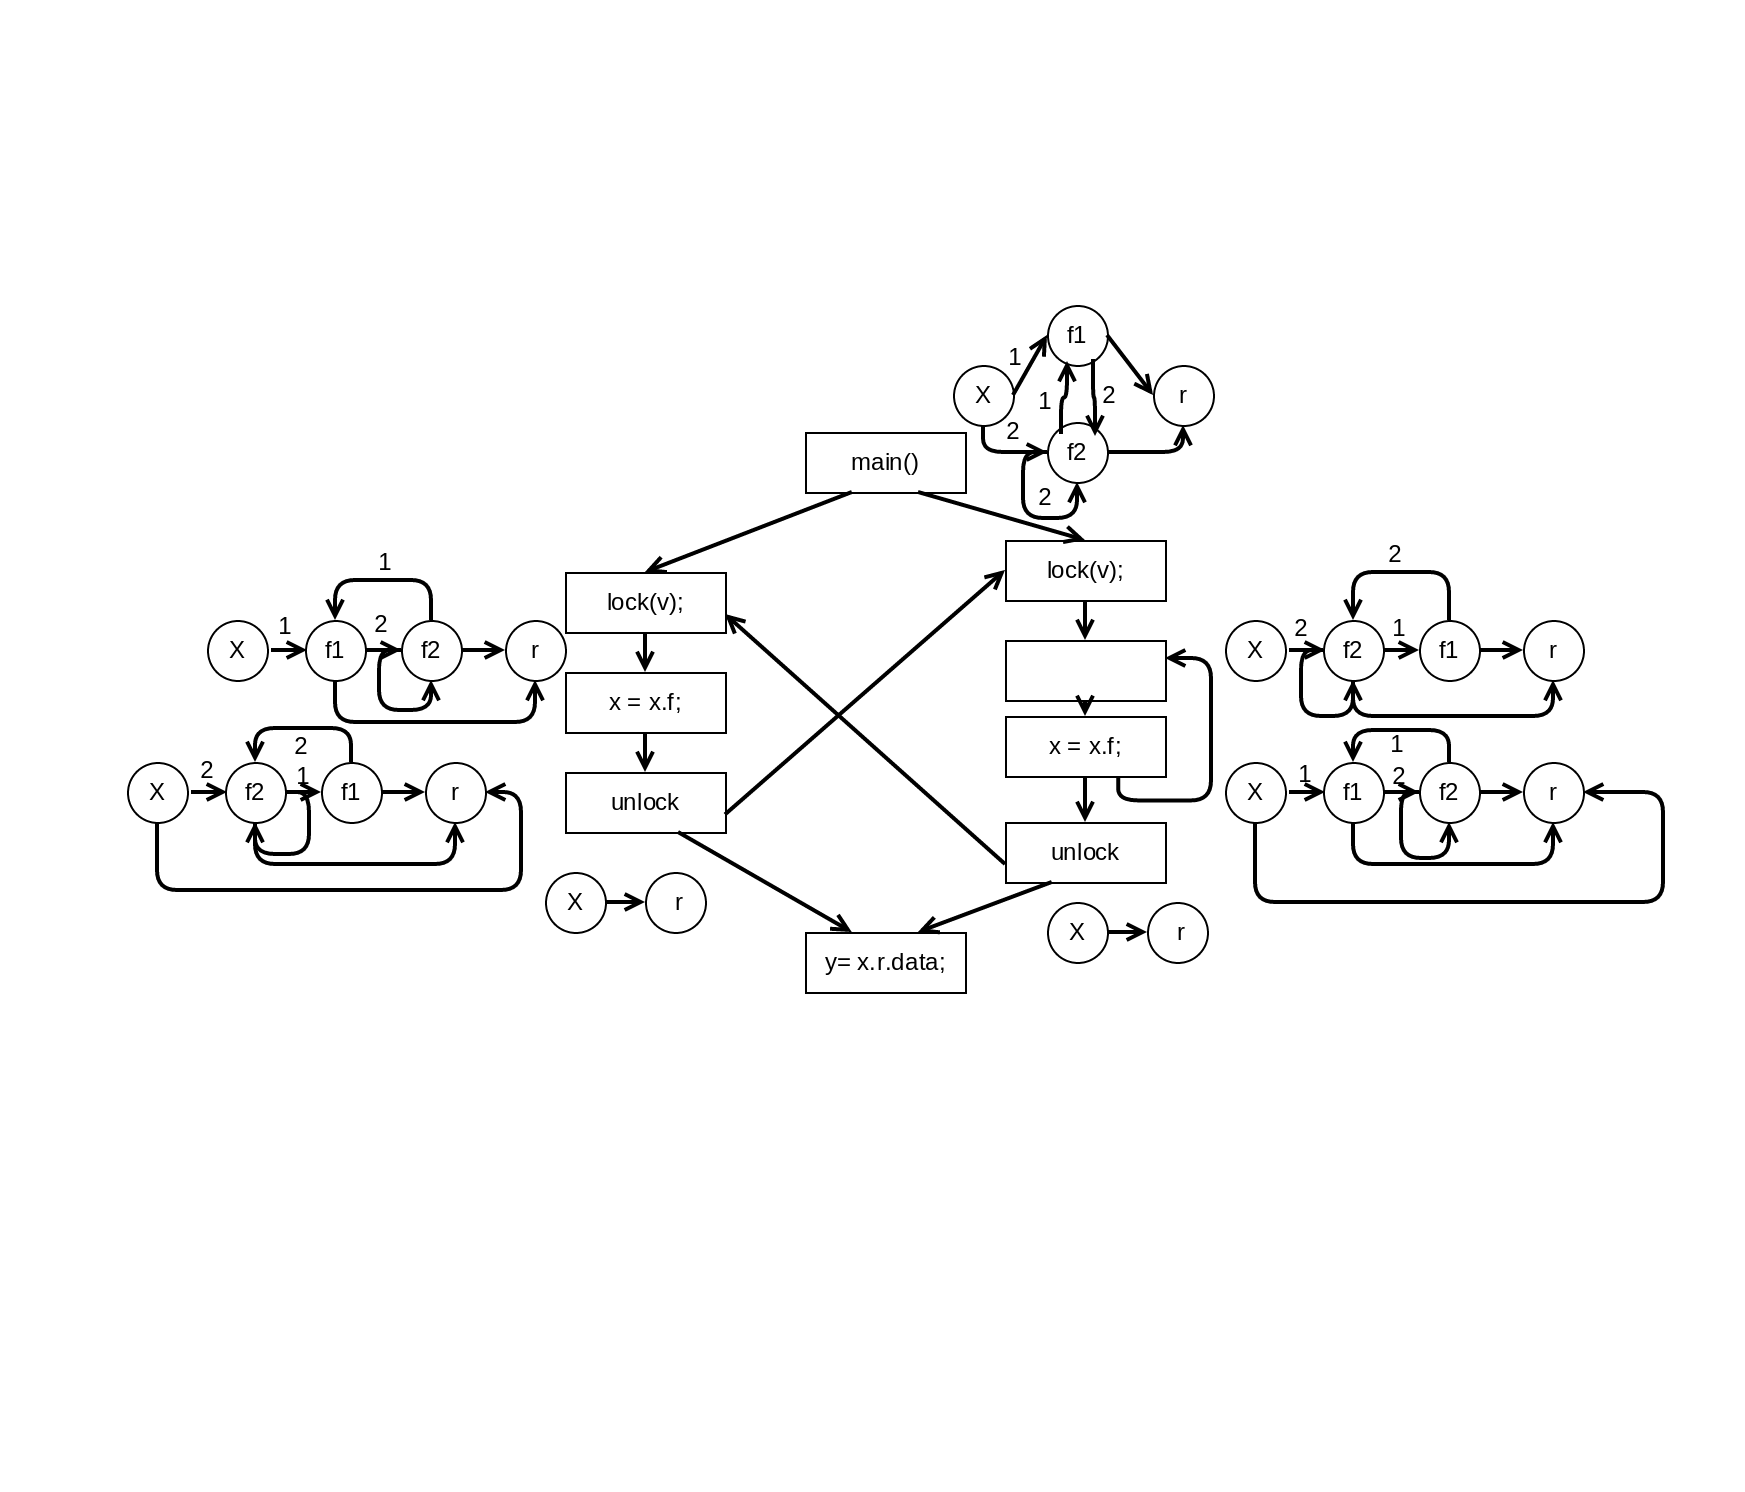
\includegraphics[width=0.8\textwidth]{Figures/crop.png}
	\caption{Concurrent Heap liveness analysis example. Note that edges are marked by thread id}
	\label{fig:threadidanalysis}
\end{figure}

          
\chapter{Tools for Design of the Analysis}

For programs with procedure call, context-sensitive analysis is required to improve the precision of data flow facts. It is needed to extend the concurrent analysis technique to inter-procedural level. In the paper, an extension based on the call strings approach was proposed. However we wish to perform inter-procedural analysis using value contexts, for better way to handle recursive programs. \\

A thread now consists of a number of procedure calls, each with their own CFGs. Each thread has an entry procedure with the same name as the thread. Execution of a thread starts with the execution of the start node of the entry procedure. Due to the inter-procedural nature we would need to handle call and return statements by adding edges from the call statement to the root node of the called procedure CFG and edges from the return statement of the called procedure CFG to the statement immediately following the call statement. \\

As an input for the concurrent inter-procedural analysis, we will supply programs with multiple threads with procedure calls in the main thread functions which can be recursive. 

\section{Call Graph Generation}

Call graph construction can be done using Soot\cite{sootguide}. The call graph is available only in whole program mode of soot (-w option). It can be accessed through the \emph{getCallGraph} method. Alternatively, call graph can also be constructed using the VASCO using the class \emph{vasco.callgraph.CallGraphTest} in the \emph{vasco.callgraph package}. VASCO generates a much precise call graph using flow and context sensitive points to analysis over the program. The arguments that need to be given along to run is the classpath containing the soot jar file, the output directory, maximum depth of call chains and the main class indicating the entry point of the program. 

The command is: \newline
\emph{java [-cp CLASSPATH] vasco.callgraph.CallGraphTest [-out DIR] [-k DEPTH] MAIN\_CLASS.} \newline

For example \\
 \emph{java -cp bin:jars/* vasco.callgraph.Test  -out "vasco-output/" -k 9 tests.test} \newline 
 is executed from the project root directory. The class file to be given as input is int the package tests.
 
For the given input program  
\begin{lstlisting}
package tests;
public class test {
	static class A {
		void foo() { bar(); }
		void bar() { }
	}

	public static void main(String[] args) {
		A a1 = new A();
		a1.foo();

		A a2 = new A();
		a2.foo();

		a2.bar();
	}
}
\end{lstlisting} 

We get the calls in the main procedure as \newline
\emph{
	PCG Method : main $\rightarrow$ foo \newline
	PCG Method : main $\rightarrow$ bar \newline
	PCG Method : main $\rightarrow$ foo \newline
	PCG Method : main $\rightarrow$ $<$init$>$ \newline
	PCG Method : main $\rightarrow$ $<$init$>$ \newline
	}

\section{Combined Unit Graph}

We will be using the \emph{CombinedUnitGraph API} to create a sync-CFG required to perform the analysis. This is currently implemented to handle 2 threads and perform intra-procedural analysis. This needs to be improved to handle more than 2 threads and construct inter-procedural CFG as discussed. \\

Creating an intra-procedural CFG :  We first create an object of the \emph{CombinedUnitGraph} class by passing the body of the 1st CFG (for the first thread) to be combined to its constructor. Then, we call the \emph{addLockUnlockUnitsForThread1} 
method to add the lock and unlock nodes in the 1st CFG and store them in respective lists. Now, we
can add the 2nd CFG to this object by calling the \emph{addGraph} method with the 2nd graph
as an argument. This is to be followed by a call to the \emph{addLockUnlockUnitsForThread2} method and finally the \emph{addUnlockToLockEdges} method call in order to complete the construction of the sync-CFG by joining unlock to lock edges for the same lock object. Exact API details are provided in the thesis on Concurrent Analysis of programs.\cite*{btpreport} \\

Consider this input program for intra-procedural live variable analysis:  
\begin{lstlisting}

import java.util.concurrent.locks.Lock;
import java.util.concurrent.locks.ReentrantLock;

public class LiveVariablesInput {
private Lock lock = new ReentrantLock();

private class Thread1 extends Thread {
	public void run() {
		int a=0,b=0;
		lock.lock();
		a = 0;
		lock.unlock();
		
		lock.lock();
		b = a;
		lock.unlock();
	}
}

private class Thread2 extends Thread {
	public void run() {
		int a=0,b=0;
		lock.lock();
		a = 0;
		lock.unlock();
		
		lock.lock();
		a = 0;
		lock.unlock();
	}
}

public static void main(String[] args) {
	LiveVariablesInput ip = new LiveVariablesInput();
	
	Thread t1 = new Thread(ip.new Thread1());
	t1.start();
	
	Thread t2 = new Thread(ip.new Thread2());
	t2.start();
	}
}
\end{lstlisting} 

The combined unit graph creates a sync-CFG in Figure 5.1 for the statements in the jimple representation of the program. The class file is converted to Jimple using Soot.

\begin{figure}
	\centering
	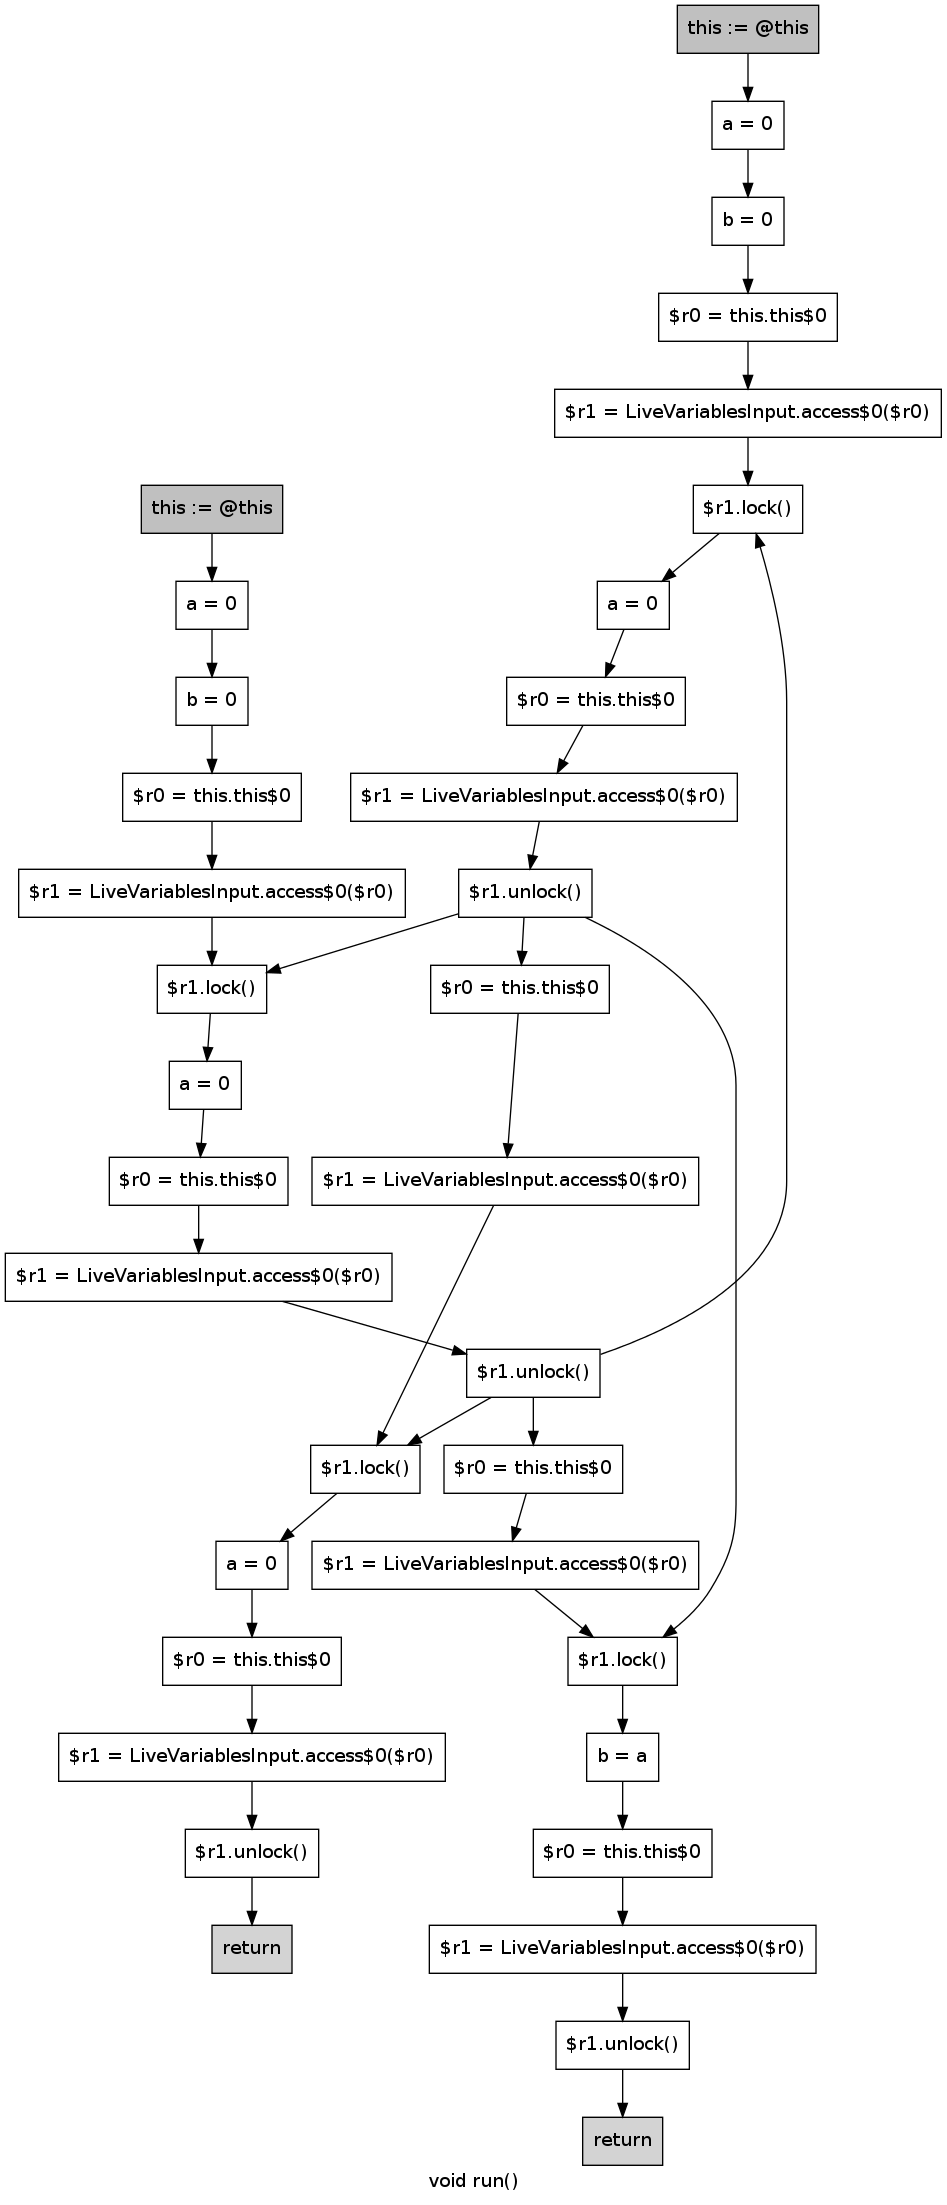
\includegraphics[width=0.6\textwidth]{Figures/combined-cfg.png}
	\caption{Sync-cfg for intra-procedural live variable analysis}
	\label{fig:live var analysis}
\end{figure} 


\section{VASCO framework}

We have already seen the use of VASCO framework to generate precise call graph for inter-procedural programs. VASCO framework is also used to design inter-procedural analysis. To perform and analysis, it is needed to override the methods \emph{normalFlowFunction, callEntryFlowFunction, callExitFlowFunction, callLocalFlowFunction, boundaryValue, copy, meet, topValue, programRepresentation} from the \emph{ForwardInterProceduralAnalysis} (or \emph{BackwardInterProceduralAnalysis} depending on the nature of the analysis).


  



 




%\chapter{Embedding Top-Down Join Enumerator}
\label{topdownint}
In this chapter we propose a new method of doing join enumeration in transformation-based optimizers based on ideas from memoization based join enumerators. DP-based and memoization-based enumeration algorithms\cite{fender2011new,fender2012effective,fender2013top} for join enumeration are more efficient in comparison to transformation-based ones in that they are able to enumerate the entire space without generating duplicates. 
In Section 6.1 we describe the algorithm, Section 6.2 describes the process for logical space generation and in  
Section 6.3 we describe a scheme for combining the two. 

\section{Conservative Partitioning}
\label{conservativePartitioning}
We describe in greater detail the conservative partitioning algorithm, denoted by \textsc{MinCutConservative} given by Pit Fender et al.\cite{fender2012effective}. The conservative partitioning algorithm is used in graph based join enumeration algorithm \textsc{TDMinCutConservative}. We try to use it here in a transformation based setting. \\

The algorithm emits all ccps for a connected vertex set $S \subseteq V$ where V is the vertex set of the query graph G=(V,E). The basic idea of conservative partitioning is to successively enhance a connected set C by members of its neighbourhood $N(C)$ at every recursive iteration. The process starts with a single vertex $t \in S$ through a redefinition of $N(\phi) = {t}$. This way, we ensure that at every instance of the algorithm's execution $C$ is connected. Since $S$ and $C \subset S$ are connected, for every possible complement $S \setminus C$ there must exist a join edge $(v1, v2)$, where $v1 \in C$ and $v2 \in (S \setminus C)$ holds. If at some point of enlarging $C$ its complement $S \setminus C$ in S is connected as well, the algorithm has found a ccp for S. \\

\begin{figure}[here]
\begin{center}
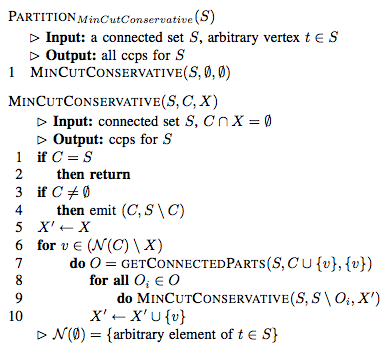
\includegraphics[width=9cm]{Figures/mincutconservative.png}
\end{center}
\caption{Pseudocode for \textsc{MinCutConservative}}
\label{fig:mincutconservative}
\end{figure}

\textsc{MinCutConservative} performs well even on when star queries are considered, where constructing every possible connected subset C of S produces an exponential overhead because most of the complements $S \setminus C$ are not connected and the partitions $(C, S \setminus C)$ computed this way are not valid ccps. Since the set C is expanded conservatively, this method remains effective. For pseudocode of the algorithm see Figure \ref{fig:mincutconservative}.

\section{Using Graph based enumeration}
We replace the existing join enumeration rules for commutativity and left associativity with a new  \textsc{N-ary Join} rule. The \textsc{N-ary Join} rule generates all ccps for the given set of n-relations. It is in essence a vanilla coated \textsc{MinCutConservative} algorithm.

\begin{defn}
A base equivalence class is defined as an equivalence class which is either a base relation or has atleast one  child logical operation node which is not a join operator.
\end{defn}

To run the \textsc{MinCutConservative} algorithm, we need the join graph induced by the base equivalence classes. For this we store two additional sets at each equivalence node:

\begin{itemize}
	\item \textsc{EqSet} : A set of all combinations of base equivalence classes being joined to generate this equivalence class. Along with this we need to store the ids of join operators of a feasible join ordering for these base equivalence class. This is used to infer the join graph.
	\item \textsc{HSet} : A set of hashes. For every set of base equivalence class that we enumerate, we generate a hash and store it in the parent equivalence class as a proof that this set has been enumerated. This is to prevent repeated enumeration of the same set of base equivalence classes.
\end{itemize}

Given with the above information, when \textsc{N-ary Join} rule is applied at a logical join operator $op$ get the \textsc{EqSet} of the left child and right child. For all combination of $S=S_{1} \cup S_{2}$ where $S_{1}\in \textsc{EqSet}_{L}$ and $S_{2}\in \textsc{EqSet}_{R}$, generate $hash(S)$ and check to ensure it has not been enumerated before. It it has not been enumerated, call \textsc{MinCutConservative}$(G_{|S})$. For every ccp generated add a new operation node to $child(parent(op))$. For every new equivalence class generated, insert it as a left-deep tree got by doing a depth-first traversal on the join graph (such a tree exists as the graph induced by these base equivalence classes is connected).

%\chapter{Future Work}
Over the course of BTP, we have identified a number of promising areas related to query optimization in transformation-based query optimizers for future work :
\begin{itemize}
	\item \textbf{Memorization based Join Enumeration} : We plan to experiment with memoization-based join enumerator as a replacement for existing join enumeration rules (see Section \ref{topdownint}). The benefits and overheads need to be analysed.
	\item \textbf{Throw in more join operators} : We plan to analyse effect of adding in more operators like left outer join, full outer join, anti join, semi join and group joins into the bucket of join operators. Even with this extended family of join operators we aim at exploring the space of all valid plans without introducing cross products. 
	\item \textbf{Sampling the Search Space} : The search space grows exponentially with respect to number of relations. The idea is to generate a sample of the search space and from this sample give the optimal plan. Galindo-Legaria et al. \cite{galindo1995uniformly} presented a method for uniform random sample of all join orders. The problems we plan to tackle :
	\begin{itemize}
		\item Random sample of space of bushy join trees
		\item Extending to generating random sample of search space even in presence of other operators
	\end{itemize}
	\item \textbf{Prioritized Search Space Exploration} : Currently the search space is explored depth first. This approach is simple, however has inherent problem that we don't assign priority for traversal of children. Pruning depends on the order of exploration and hence it might be beneficial to assign 'priority' to each of the children and choose order based on this. Some ideas in \cite{fender2012effective}.	
	\item \textbf{Extending to Cascades and Columbia}: The Cascades optimizer generator overcomes many of the shortcomings of Volcano. We wish to check the applicability of things discussed in this report for use in Cascades style framework.	
\end{itemize}
\chapter{Conclusion and Future Work}

In this report the topics covered are : 

\begin{itemize}
	\item The mechanism of Heap reference analysis using points-to and live variable analysis on access paths. It is necessary to store the access path values at a statement as an access graph to keep the data fact bounded.
	\item The method of value context used to carry out precise inter-procedural analysis with an example case on handling recursion.
	\item The technique of constructing sync-cfg for performing intra-procedural data flow analysis of concurrent programs.
	\item The extension of concurrent analysis to an inter-procedural level, by using VASCO for generating call-graph and designing inter-procedural analysis.
\end{itemize}

The future work to be done is:

\begin{itemize}
	\item Implementation of CombinedUnitGraph class to handle programs with more than 2 threads.
	\item Using Value context method of performing inter-procedural analysis on data-race free concurrent programs containing function calls.
	\item Implementing Heap reference analysis on concurrent programs containing function calls.
\end{itemize}

%\cite{liveness}\cite{slides}\cite{liveness}\cite{hra}\cite{btpreport}\cite{sootguide}\cite{Arnab2006}\cite{mtpreport}
%\pagenumbering{roman}

\printbibliography [heading=bibintoc]



\end{document}
